\newpage
\chapter*{\centering{\MakeUppercase{PHẦN 3: THỰC NGHIỆM VÀ PHÂN TÍCH ĐÁNH GIÁ}}}
\phantomsection
\addcontentsline{toc}{chapter}{\textcolor{fitblue}{\MakeUppercase{PHẦN 3: THỰC NGHIỆM VÀ PHÂN TÍCH ĐÁNH GIÁ}}}

\section*{3.1. Giới thiệu tổng quan và Cơ sở lý thuyết}
\phantomsection
\addcontentsline{toc}{section}{3.1. Giới thiệu tổng quan và Cơ sở lý thuyết}

Mục tiêu của phần này là khảo sát, đo lường và đánh giá ba thuật toán giải hệ phương trình tuyến tính $Ax = b$ phổ biến: Khử Gauss, Phân rã QR, và Lặp Gauss-Seidel. Quá trình đánh giá được thực hiện qua hai lăng kính chính: hiệu năng phần mềm (như thời gian thực thi) và tính ổn định số học (sai số làm tròn trên không gian dấu phẩy động).

Theo yêu cầu của đề tài, toàn bộ thuật toán được \textbf{tự lập trình bằng Python thuần} bằng cấu trúc dữ liệu `list of lists` (không sử dụng \texttt{numpy.linalg.solve} hay ma trận `numpy.ndarray` c-extension). Điều này đảm bảo chi phí tính toán lý thuyết và thực tế được phản xạ một cách trung thực nhất.

\textbf{Cơ sở lý thuyết dùng để đánh giá:}
\begin{itemize}
    \item \textbf{Sai số dư tương đối:} Là thước đo độ chính xác của nghiệm tìm được $\hat{x}$ so với vế phải của phương trình bằng chuẩn 2:
    $$ \text{Sai số dư tương đối} = \frac{\|A\hat{x} - b\|_2}{\|b\|_2} $$
    \item \textbf{Độ phức tạp tính toán:} Số phép toán dấu phẩy động (FLOPs). Phân rã trực tiếp (Gauss, QR) đòi hỏi $O(n^3)$ thời gian, trong khi Gauss-Seidel có thể đạt xấp xỉ $O(k n^2)$ nếu hội tụ sau $k$ bước lặp.
    \item \textbf{Số điều kiện và Định lý sai số:} Kí hiệu $\kappa(A) = \|A\| \cdot \|A^{-1}\|$. Đây là đại lượng mô tả mức khuếch đại sai số của hệ phương trình. Định lý sai số cho biết mối quan hệ giữa sai số tương đối của nghiệm (sai số thuận - Forward Error, $\|\Delta x\|/\|x\|$) và sai số tương đối của dữ liệu đầu vào (sai số ngược - Backward Error, $\|\Delta b\|/\|b\|$) qua bất đẳng thức:
    $$ \frac{\|\Delta x\|}{\|x\|} \leq \kappa(A) \cdot \frac{\|\Delta b\|}{\|b\|}. $$
    \item \textbf{Phân rã ma trận lặp:} Với Gauss-Seidel, ta viết $A = D + L + U$ (trong đó $D$ là đường chéo, $L$ là tam giác dưới thuần, $U$ là tam giác trên thuần). Công thức lặp:
    $$ x^{(k+1)} = -(D+L)^{-1}U x^{(k)} + (D+L)^{-1}b. $$
    Dạng theo từng thành phần:
    $$ x_i^{(k+1)} = \frac{1}{a_{ii}}\left(b_i - \sum_{j=1}^{i-1} a_{ij} x_j^{(k+1)} - \sum_{j=i+1}^{n} a_{ij} x_j^{(k)}\right). $$
    Điều kiện hội tụ đủ: ma trận chéo trội chặt theo hàng, tức $|a_{ii}| > \sum_{j \ne i} |a_{ij}|$.
\end{itemize}

\textbf{Bảng so sánh các phương pháp:}
\begin{table}[H]
    \centering
    \caption{So sánh đặc trưng các phương pháp giải hệ tuyến tính}
    \vspace{0.2cm}
    \renewcommand{\arraystretch}{1.2}
    \begin{tabular}{|l|c|l|c|c|}
    \hline
    \textbf{Phương pháp} & \textbf{Loại} & \textbf{Điều kiện áp dụng} & \textbf{Chi phí} & \textbf{Ổn định} \\ \hline
    Gauss (Partial Pivoting) & Trực tiếp & Mọi $A$ khả nghịch & $O(n^3)$ & Cao \\ \hline
    QR (Gram-Schmidt) & Trực tiếp & Mọi $A$ (kể cả chữ nhật) & $O(n^3)$ & Rất cao \\ \hline
    Gauss--Seidel & Lặp & Chéo trội hàng / SPD & $O(k n^2)$ & Trung bình \\ \hline
    \end{tabular}
\end{table}

\section*{3.2. Cài đặt thuật toán giải hệ phương trình tuyến tính}
\phantomsection
\addcontentsline{toc}{section}{3.2. Cài đặt thuật toán giải hệ phương trình tuyến tính}

Khối mã giả dưới đây chi tiết hóa quy trình thực thi của 3 thuật toán nền tảng. Các thuật toán được thiết kế để xử lý dữ liệu đầu vào là ma trận vuông $A$ và vector $b$, trả về nghiệm tối ưu $x$ tiệm cận với nghiệm thực tế của hệ phương trình.

\subsection*{3.2.1. Phương pháp Khử Gauss (Partial Pivoting)}
\phantomsection
\addcontentsline{toc}{subsection}{3.2.1. Phương pháp Khử Gauss (Partial Pivoting)}

Thuật toán khử Gauss là phương pháp trực tiếp, bản chất biến đổi hệ phương trình gốc về dạng tam giác trên để giải bằng thế ngược. Việc áp dụng cơ chế Partial Pivoting (chọn phần tử chốt lớn nhất theo trị tuyệt đối trên cột khử hiện tại, rồi hoán vị hàng) là bắt buộc để đảm bảo tính ổn định số học.

\begin{algorithm}[H]
\caption{Giải hệ phương trình bằng Khử Gauss (Partial Pivoting)}
\label{alg:gauss_pivoting}
\begin{algorithmic}[1]
\Procedure{SOLVE\_GAUSS}{$A, b$}
    \State $n \gets \text{size}(A)$
    \For{$i \gets 0$ to $n-1$}
        \State $max\_row \gets i$; $max\_val \gets |A[i][i]|$
        \For{$k \gets i+1$ to $n-1$} \Comment{Tìm phần tử chốt lớn nhất}
            \If{$|A[k][i]| > max\_val$}
                \State $max\_val \gets |A[k][i]|$; $max\_row \gets k$
            \EndIf
        \EndFor
        \State Hoán vị hàng $i$ và $max\_row$ cho cả $A$ và $b$
        \For{$k \gets i+1$ to $n-1$} \Comment{Khử các dòng phía dưới}
            \State $factor \gets A[k][i] / A[i][i]$
            \For{$j \gets i+1$ to $n-1$}
                \State $A[k][j] \gets A[k][j] - factor \times A[i][j]$
            \EndFor
            \State $b[k] \gets b[k] - factor \times b[i]$
        \EndFor
    \EndFor
    \State $x \gets$ giải bằng thế ngược từ $A$ và $b$ đã khử tam giác
    \State \Return $x$
\EndProcedure
\end{algorithmic}
\end{algorithm}

\subsection*{3.2.2. Phương pháp Phân rã QR (Gram-Schmidt)}
\phantomsection
\addcontentsline{toc}{subsection}{3.2.2. Phương pháp Phân rã QR (Gram-Schmidt)}

Ứng dụng thuật toán trực giao hóa Gram-Schmidt để phân rã ma trận gốc thành tích $A = QR$ (với $Q$ là ma trận trực giao và $R$ là ma trận tam giác trên). So với Gauss phụ thuộc vào pivoting, hướng tiếp cận QR ổn định hơn, đặc biệt đối với các ma trận có số điều kiện lớn. Bài toán được giải thông qua hệ trung gian $Rx = Q^Tb$.

\begin{algorithm}[H]
\caption{Giải hệ phương trình bằng Phân rã QR (Gram-Schmidt)}
\label{alg:solve_qr}
\begin{algorithmic}[1]
\Procedure{SOLVE\_QR}{$A, b$}
    \State $n \gets \text{size}(A)$
    \State $Q, R \gets \text{Ma trận không } n \times n$
    \For{$j \gets 0$ to $n-1$} \Comment{Quy trình Gram-Schmidt cải tiến}
        \State $v \gets A[0 \dots n-1][j]$
        \For{$i \gets 0$ to $j-1$}
            \State $R[i][j] \gets \sum_{k=0}^{n-1} Q[k][i] \times v[k]$
            \State $v \gets v - R[i][j] \times Q[0 \dots n-1][i]$
        \EndFor
        \State $R[j][j] \gets \|v\|_2$
        \State $Q[0 \dots n-1][j] \gets v / R[j][j]$
    \EndFor
    \State $y \gets Q^T b$
    \State $x \gets$ giải thế ngược từ $Rx = y$
    \State \Return $x$
\EndProcedure
\end{algorithmic}
\end{algorithm}

\subsection*{3.2.3. Phương pháp Lặp Gauss-Seidel}
\phantomsection
\addcontentsline{toc}{subsection}{3.2.3. Phương pháp Lặp Gauss-Seidel}

Trái với hai phương pháp trực tiếp, Gauss-Seidel là thuật toán lặp: bắt đầu với một đoán trước ban đầu $x^{(0)} = \vec{0}$, thuật toán thay thế nghiệm mới tức thời vào bên trong mô hình để sinh ra nghiệm hội tụ. Phương pháp này chỉ thành công khi ma trận đạt tính chất đường chéo trội nghiêm ngặt hoặc đối xứng xác định dương.

\begin{algorithm}[H]
\caption{Giải hệ phương trình bằng Lặp Gauss-Seidel}
\label{alg:gauss_seidel}
\begin{algorithmic}[1]
\Procedure{GAUSS\_SEIDEL}{$A, b, max\_iters, tol$}
    \State $x \gets$ mảng $n$ phần tử 0; $n \gets$ cấp của $A$
    \For{$it \gets 1$ to $max\_iters$}
        \State $max\_diff \gets 0$
        \For{$i \gets 0$ to $n-1$}
            \State $s \gets \sum_{j \neq i} A[i][j] \times x[j]$
            \State $x_{new} \gets (b[i] - s) / A[i][i]$
            \State $max\_diff \gets \max(max\_diff, |x_{new} - x[i]|)$
            \State $x[i] \gets x_{new}$
        \EndFor
        \If{$max\_diff < tol$}
            \State \textbf{break} \Comment{Hội tụ}
        \EndIf
    \EndFor
    \State \Return $x$
\EndProcedure
\end{algorithmic}
\end{algorithm}

\section*{3.3. Thực nghiệm đo lường hiệu năng và phân tích}
\phantomsection
\addcontentsline{toc}{section}{3.3. Thực nghiệm đo lường hiệu năng và phân tích}

Để đánh giá độ phức tạp thời gian theo kích thước bài toán, nhóm sinh ngẫu nhiên các ma trận vuông chéo trội nghiêm ngặt nhằm đảm bảo hội tụ của Gauss--Seidel. Tập kích thước thử nghiệm là $n \in \{50, 100, 200, 500, 1000\}$. Thời gian được đo bằng \texttt{time.perf\_counter()}; với $n < 500$ chạy $5$ lần lấy trung bình, với $n = 500, 1000$ chạy $1$ lần để tránh thời gian quá dài.

\textbf{Bảng thống kê kết quả chạy thực nghiệm (trích xuất từ cấu hình đo lường Notebook):}
\begin{table}[H]
    \centering
    \caption{So sánh thời gian chạy thực tế (s) và sai số dư tương đối theo các hệ $N$}
    \vspace{0.2cm}
    \renewcommand{\arraystretch}{1.3}
    \resizebox{\textwidth}{!}{
        \begin{tabular}{|c|c|c|c|c|c|c|}
        \hline
        \textbf{Cấp $n$} & \textbf{Khử Gauss Time} & \textbf{Sai số dư Gauss} & \textbf{QR Time} & \textbf{Sai số dư QR} & \textbf{G-Seidel Time} & \textbf{Sai số dư GS} \\ \hline
        50   & 0.002820 s & $1.90 \times 10^{-16}$ & 0.010590 s & $1.24 \times 10^{-16}$ & \textbf{0.002894 s} & $4.84 \times 10^{-11}$ \\ \hline
        100  & 0.020056 s & $2.97 \times 10^{-16}$ & 0.079861 s & $1.39 \times 10^{-16}$ & \textbf{0.011074 s} & $7.17 \times 10^{-11}$ \\ \hline
        200  & 0.159520 s & $3.69 \times 10^{-16}$ & 0.856179 s & $1.89 \times 10^{-16}$ & \textbf{0.045281 s} & $5.60 \times 10^{-11}$ \\ \hline
        500  & 2.971386 s & $6.67 \times 10^{-16}$ & 12.450867 s & $2.58 \times 10^{-16}$ & \textbf{0.295427 s} & $7.12 \times 10^{-11}$ \\ \hline
        1000 & 27.374951 s & $9.95 \times 10^{-16}$ & 111.553300 s & $3.18 \times 10^{-16}$ & \textbf{1.256143 s} & $8.07 \times 10^{-11}$ \\ \hline
        \end{tabular}
    }
\end{table}

\begin{figure}[H]
    \centering
    % Lưu ảnh log_log_plot.png vào folder images
    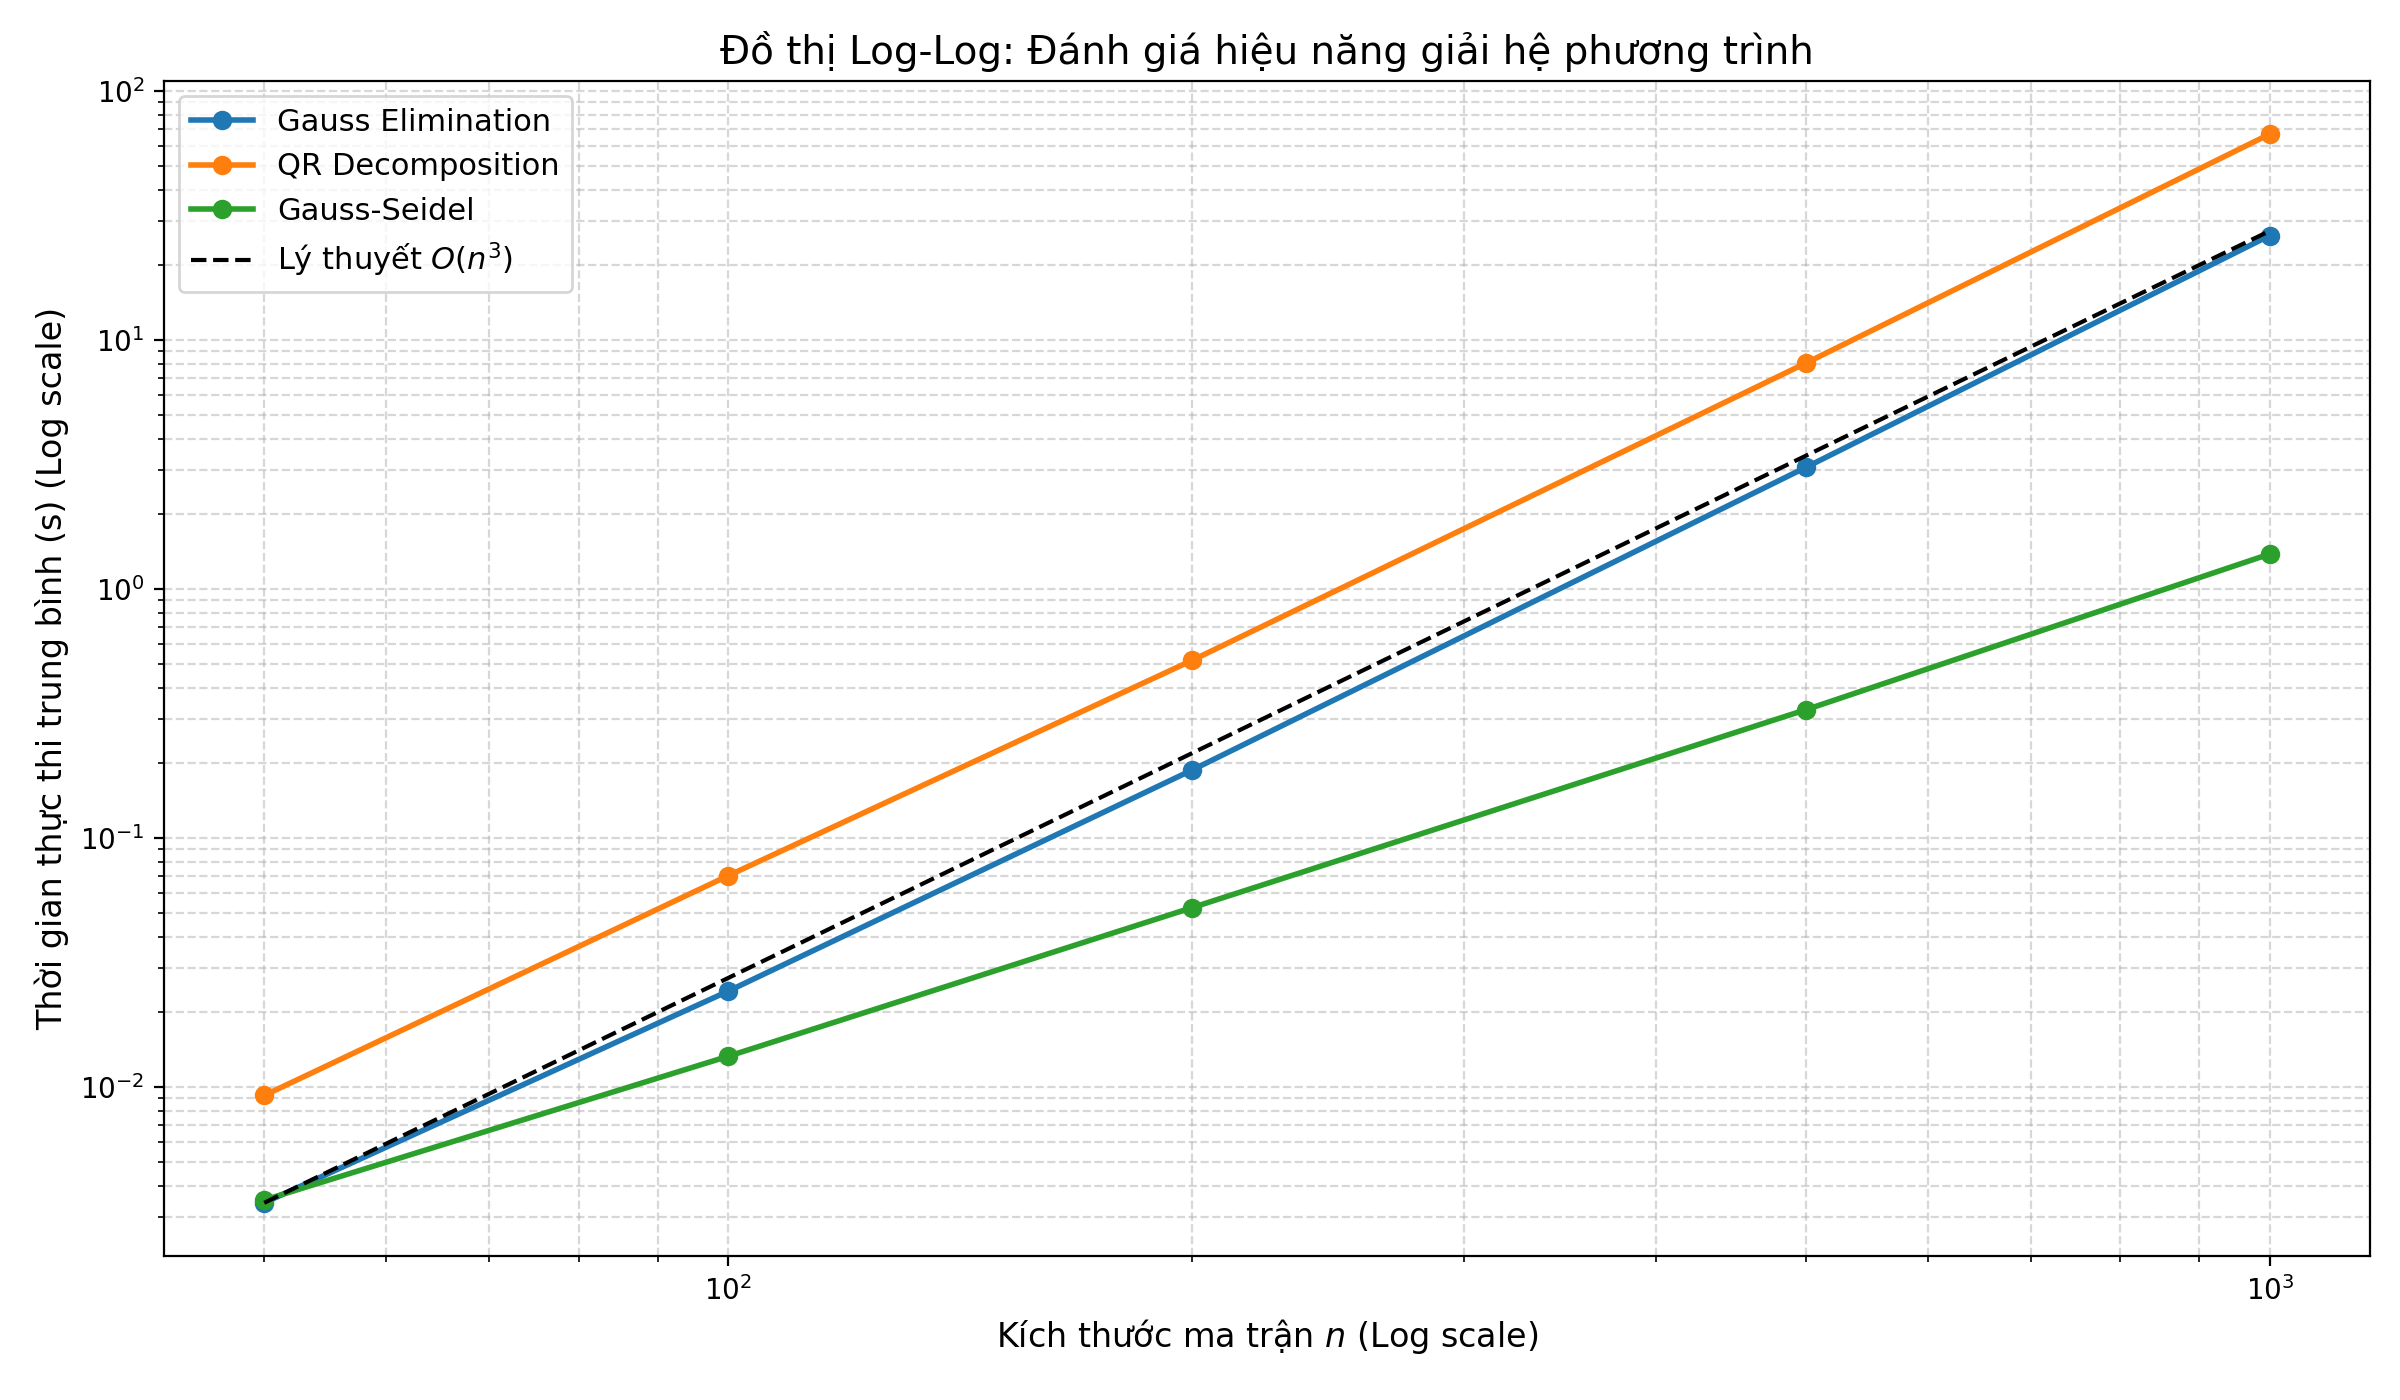
\includegraphics[width=0.8\textwidth]{images/log_log_plot.png}
    \caption{Đồ thị Log-Log mô phỏng trực quan thời gian chạy của ba phương pháp}
\end{figure}

Việc vẽ đồ thị theo nguyên lý Logarit cơ số kép (Log-Log plot) biến các đường cong đa thức $T(n) = c \cdot n^\alpha$ thành các đường thẳng có hệ số góc bằng hệ số mũ $\alpha$, giúp ta dễ dàng tính được bậc độ phức tạp lý thuyết thực tế. Từ đồ thị trên và các số liệu thuộc bảng kiểm nghiệm, ta trực tiếp rút ra ba nhóm kết luận khoa học vững chắc:

\subsection*{3.3.1. Phân tích Khử Gauss (Partial Pivoting)}
Đường đo lường trên không gian log-log bám sát lý thuyết $O(n^3)$ (hệ số góc $\alpha \approx 3$). Phương pháp mất khoảng $27.37$ giây để giải hệ $n=1000$, đồng thời duy trì sai số dư tương đối quanh mức $10^{-16}$, tiệm cận giới hạn máy chính xác (machine epsilon) của float64. Kỹ thuật partial pivoting giúp ổn định quá trình khử và tránh chia cho phần tử chốt quá nhỏ.

\subsection*{3.3.2. Phân tích Phân rã QR (Gram-Schmidt)}
Mặc dù có cùng hệ số góc $\alpha \approx 3$, thời gian thực thi của QR luôn cao hơn Gauss. Ở $n=1000$, QR tốn $111.55$ giây, lớn hơn khoảng $4.07$ lần so với Gauss. Lý do đến từ chi phí trực giao hóa trong Gram-Schmidt, vốn có hằng số lớn hơn trong $O(n^3)$. Đổi lại, QR ổn định hơn khi ma trận gần suy biến.

\subsection*{3.3.3. Hiệu năng của phương pháp lặp Gauss-Seidel}
Đường Gauss--Seidel có độ dốc nhỏ hơn so với hai phương pháp trực tiếp. Với $n=1000$, thời gian là $1.26$ giây. Kết quả này đến từ việc mỗi vòng lặp chỉ tốn $O(n^2)$ phép tính; khi ma trận chéo trội nghiêm ngặt, số vòng lặp hội tụ $k$ không quá lớn, dẫn đến chi phí tổng quát $O(k n^2)$.

\subsection*{3.3.4. Phân tích chi phí tính toán và Truy xuất Bộ nhớ}
Việc phân giải cơ chế thời gian thực thi của các phương pháp trên không chỉ dựa vào mô hình Toán lý thuyết mà còn phụ thuộc vào kiến trúc phần cứng máy tính. Về chi phí tính toán (FLOPs), thuật toán Gauss cơ bản yêu cầu xấp xỉ $\frac{2}{3}n^3$ phép nhân-cộng dấu phẩy động; trong khi kịch bản trực giao hóa của thuật giải Gram-Schmidt (QR) tiến hành $\approx 2n^3$ thao tác liên kết tổng vector và bình phương Euclidean. 

Thực tế ghi nhận sự chênh lệch thời gian ở $N=1000$ là $(111.55/27.37) \approx 4.07$ lần. Sự khác biệt này đến từ chi phí trực giao hóa trong QR và cách truy xuất bộ nhớ. Với \texttt{list of lists}, truy xuất theo cột trong QR kém liên tục hơn so với truy xuất theo hàng trong Gauss, làm tăng độ trễ truy xuất bộ nhớ.
\section*{3.4. Phân tích tính ổn định số học: Ma trận Hilbert vs. SPD}
\phantomsection
\addcontentsline{toc}{section}{3.4. Phân tích tính ổn định số học: Ma trận Hilbert vs. SPD}

Độ chính xác của hệ phương trình $Ax = b$ không chỉ phụ thuộc vào cơ chế thuật toán, mà còn vấp vào đặc thù cấu trúc toán học của bản thân ma trận $A$. Phép đánh giá này được thực hiện để chứng minh vấn đề về sai số do hiện tượng làm tròn (round-off error) đối với các hệ thống có tính đa cộng tuyến cao – được đánh giá thông qua chỉ số của Số điều kiện $\kappa(A)$.

\subsection*{3.4.1. Thiết lập biến cố thực nghiệm}
Nhóm đối chiếu sai số dư của hai dạng ma trận vuông với kích thước cơ sở $n=10$:
\begin{itemize}
    \item \textbf{Ma trận Hilbert ($H_n$):} Khởi tạo dưới dạng $H_{ij} = \frac{1}{i+j-1}$. Ma trận này được biết đến với cấu trúc đặc trưng thiếu điều kiện số học hay hệ điều kiện kém (ill-conditioned) do khoảng cách giữa các vector cột vô cùng gần nhau.
    \item \textbf{Ma trận Đối xứng Xác Định Dương (SPD):} Khởi tạo bằng phép nhân $A = X^T X + nI$ để bảo đảm tính xác định dương.
\end{itemize}
Đối với Gauss--Seidel, điều kiện hội tụ đủ là chéo trội; tuy nhiên với ma trận SPD, phương pháp vẫn hội tụ theo lý thuyết, dù không nhất thiết thỏa chéo trội theo hàng.
Trong thí nghiệm này, số điều kiện được trình bày theo $\kappa(A)$ như trong notebook thực nghiệm.

\begin{table}[H]
    \centering
    \caption{Sai số dư và số điều kiện (chuẩn vô cùng) với $N=10$}
    \vspace{0.2cm}
    \renewcommand{\arraystretch}{1.3}
    \begin{tabular}{|c|c|c|c|c|}
    \hline
    \textbf{Loại ma trận} & \textbf{Số điều kiện $\kappa(A)$} & \textbf{Sai số dư Gauss} & \textbf{Sai số dư QR} & \textbf{Sai số dư GS} \\ \hline
    Hilbert (Ill-conditioned) & $1.60 \times 10^{13}$ & $0.00$ & $2.20 \times 10^{-6}$ & $4.19 \times 10^{-6}$ \\ \hline
    SPD (Well-conditioned) & $2.20$ & $1.96 \times 10^{-16}$ & $2.10 \times 10^{-16}$ & $1.22 \times 10^{-11}$ \\ \hline
    \end{tabular}
\end{table}

\begin{figure}[H]
    \centering
    % Lưu ảnh condition_number_plot.png từ IPython Jupyter Data
    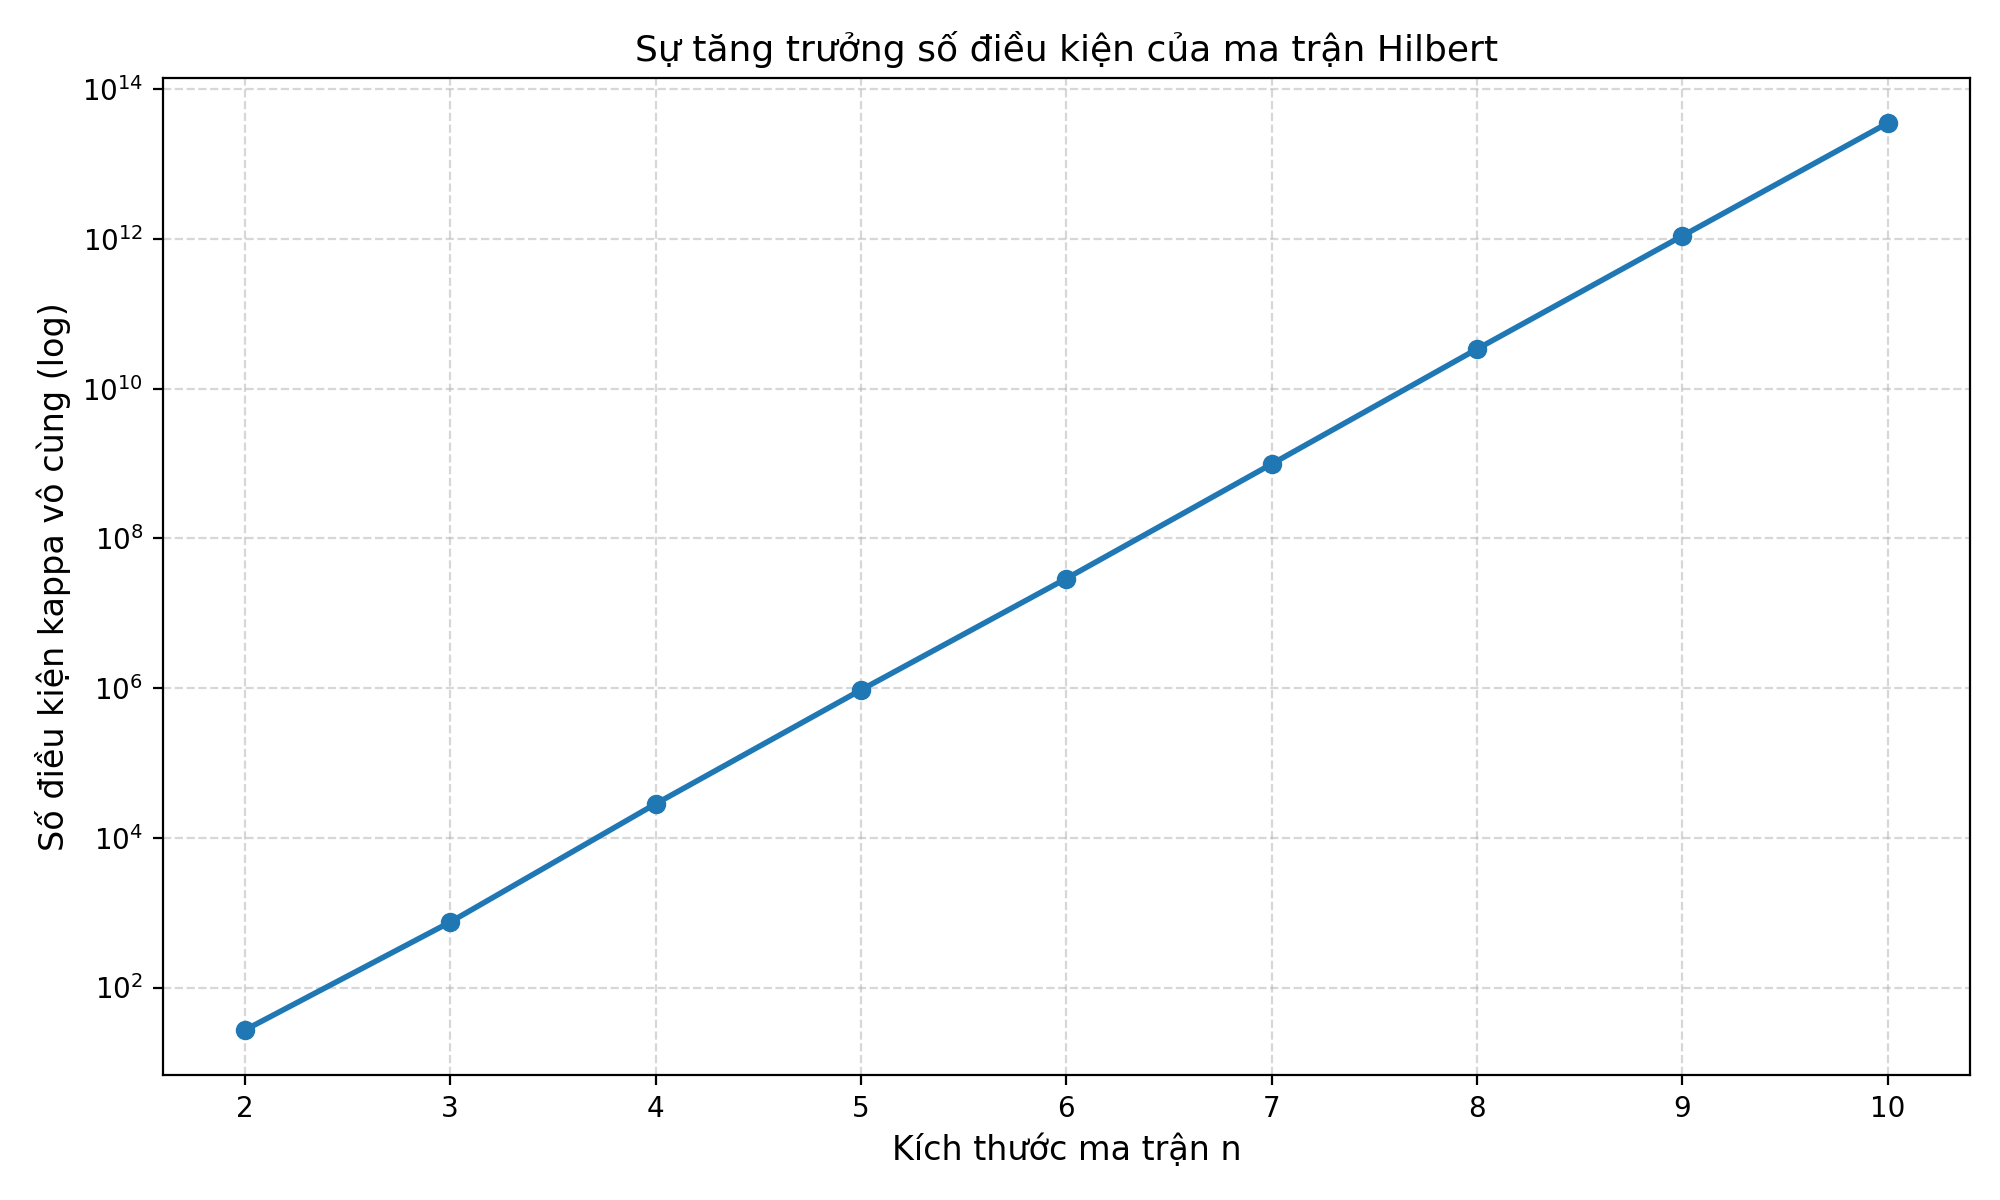
\includegraphics[width=0.8\textwidth]{images/condition_number_plot.png}
    \caption{Biểu đồ phân tích độ khuếch đại của số điều kiện Hilbert khi kích thước ma trận n gia tăng}
\end{figure}

\subsection*{3.4.2. Phân tích sai số theo số điều kiện}
Ma trận Hilbert có $\kappa(A)$ rất lớn ($\approx 1.6 \times 10^{13}$), dẫn đến sai số dư của QR và Gauss--Seidel ở mức $10^{-6}$. Trong khi đó, ma trận SPD có $\kappa(A)$ nhỏ ($\approx 2.2$), nên cả Gauss và QR đều đạt sai số dư gần $10^{-16}$. Kết quả này phù hợp với lý thuyết sai số: khi $\kappa(A)$ lớn, sai số bị khuếch đại đáng kể ngay cả khi thuật toán ổn định.

Ở trường hợp SPD, Gauss--Seidel vẫn cho sai số dư lớn hơn hai phương pháp trực tiếp. Nguyên nhân chính là đây là phương pháp lặp với ngưỡng dừng hữu hạn, nên sai số dư không thể tiệm cận máy chính xác như Gauss và QR.

\subsection*{3.4.3. Kết luận về tính ổn định của thuật toán}
Kết quả thực nghiệm cho thấy việc \textbf{kiểm định số điều kiện} là bước bắt buộc trước khi giải hệ tuyến tính. Các ma trận ill-conditioned như Hilbert có thể làm mất độ tin cậy của nghiệm ngay cả với kích thước nhỏ. Điều này khẳng định rằng tối ưu hóa mã nguồn không thể thay thế cho việc đánh giá điều kiện của bài toán.

\section*{3.5. Chỉ dẫn lựa chọn giải thuật}
Dựa trên sự cân bằng giữa chi phí thực thi và độ ổn định số học, nhóm đề xuất quy trình lựa chọn thuật toán giải hệ $Ax = b$ như sau:

\begin{itemize}
    \item \textbf{Phương pháp Khử (Gauss / LU / Cholesky):} Ưu tiên sử dụng cho các ma trận đặc (Dense Matrices) có kích thước từ nhỏ đến trung bình (dưới 10.000 ẩn số) và có số điều kiện thấp ($\kappa(A) < 10^3$). Đây là lựa chọn tối ưu về mặt tốc độ trong điều kiện ma trận ổn định.
    \item \textbf{Phương pháp Trực giao (QR):} Áp dụng cho các bài toán yêu cầu độ ổn định số học cao hoặc các hệ phương trình không vuông (mô hình hồi quy, Bình phương tối thiểu). Mặc dù chi phí thời gian cao hơn, QR đảm bảo tính chính xác cho các hệ có nguy cơ nhiễu số học.
    \item \textbf{Phương pháp Lặp (Gauss-Seidel):} Là lựa chọn hàng đầu cho các ma trận thưa quy mô lớn (Sparse Matrices với tỷ lệ phần tử khác 0 thấp), ma trận đường chéo trội hoặc các hệ phương trình đạo hàm riêng (PDEs). Phương pháp này tối ưu hóa việc sử dụng bộ nhớ và thời gian tính toán thông qua cơ chế hội tụ dần.
\end{itemize}
